\documentclass[10pt]{article}

%\def\python{}


\usepackage[utf8]{inputenc}

\usepackage{tabularx}
\usepackage{amsmath}
\usepackage{amssymb}
\usepackage{geometry}
\geometry{a4paper, top=25mm, left=30mm, right=25mm, bottom=30mm,
         headsep=10mm, footskip=12mm}

\usepackage{graphicx}
\usepackage{url}

\usepackage{graphicx}
\usepackage[pdftex,colorlinks=true,citecolor=blue,urlcolor=blue,linkcolor=blue]{hyperref}
\usepackage{color}
\usepackage{xcolor}
\usepackage{tabularx}
\usepackage{listings}
\usepackage{parcolumns}
\usepackage{longtable}
\usepackage[margin=10pt]{caption}

% set the title
\title{\begin{tabular}{p{11cm}}\centering
Face Recognition with OpenCV2
\end{tabular}}

% contact details
\author{Philipp Wagner\\\href{http://www.bytefish.de}{http://www.bytefish.de}}

% colors for syntax highlightning
\definecolor{darkblue}{rgb}{0,0,.6}
\definecolor{darkred}{rgb}{.6,0,0}
\definecolor{darkgreen}{rgb}{0,.6,0}
\definecolor{red}{rgb}{.98,0,0}


% Listings Style
\lstset{
	numberstyle=\footnotesize, 
	basicstyle=\footnotesize\ttfamily
	numbers=left, 
	numbersep=5pt, 
	frame=single
}

% Add basic syntax highlightning to C++
\lstset{
	numberstyle=\footnotesize, 
	basicstyle=\footnotesize\ttfamily,
	numbers=none, 
	numbersep=5pt, 
	frame=single,
	breaklines=true,
	showspaces=false,
	showstringspaces=false,
	showtabs=false,
	tabsize=2,
}

\lstloadlanguages{C++}
\lstset{
	language=C++,
  commentstyle=\footnotesize\ttfamily\color{darkgreen},
  keywordstyle=\footnotesize\ttfamily\color{darkblue},
  stringstyle=\footnotesize\ttfamily\color{darkred},
}

\lstdefinelanguage{cmake}{
	morekeywords={cmake_minimum_required, project, find\_package, add\_executable, target\_link\_libraries},
	sensitive=false,
	morecomment=[l]{\#},
}

% change vertical space of itemize, description and enumeration environments
\let\olditemize=\itemize
   \def\itemize{\olditemize\setlength{\itemsep}{-0.5ex}}
\let\oldenumerate=\enumerate
   \def\enumerate{\oldenumerate\setlength{\itemsep}{-0.5ex}}
\let\olddescription=\description
   \def\description{\olddescription\setlength{\itemsep}{-0.5ex}}
   
% don't indent sections
\setlength{\parindent}{0pt}

\begin{document}

\maketitle

\section{Introduction}

\href{http://opencv.willowgarage.com}{OpenCV (Open Source Computer Vision)} is a popular computer vision library started by \href{http://www.intel.com}{Intel} in 1999. The cross-platform library sets its focus on real-time image processing and includes patent-free implementations of the latest computer vision algorithms. In 2008 \href{http://www.willowgarage.com}{Willow Garage} took over support and OpenCV 2.3.1 now comes with a programming interface to C, C++, \href{http://www.python.org}{Python} and \href{http://www.android.com}{Android}. OpenCV is released under a BSD license, so it is used in academic and commercial projects such as \href{http://www.google.com/streetview}{Google Streetview}.

This document is the guide I've wished for, when I was working myself into face recognition. It helps you with installing OpenCV2 on your machine and explains you how to build a project on Windows and Linux. Two face recognition algorithms are prototyped with \ifx\python\undefined \href{http://www.gnu.org/software/octave/}{GNU Octave}/\href{http://www.mathworks.com}{MATLAB} \else \href{http://www.python.org}{Python}\fi{} and implemented with the OpenCV2 C++ API. All concepts are explained in detail, but a basic knowledge of C++ is assumed. I've decided to leave the C++ implementation details out (as I am afraid they confuse people) and provide you with examples how to use the projects. \href{http://www.mingw.org}{MinGW} (the GCC port for Windows) is used as the C/C++ compiler for Windows, because it works great with OpenCV2 and comes under terms of a public license (please see \href{http://www.mingw.org/license}{mingw.org/license} for details). If someone writes a similar guide for Microsoft Visual Studio 2008/2010, I would be happy to add it to the document.

You don't need to copy and paste the code snippets, the code has been pushed into my github repository:

\begin{itemize}
  \item \href{http://www.github.com/bytefish}{github.com/bytefish}
  \item \href{http://www.github.com/bytefish/facerecognition_guide}{github.com/bytefish/facerecognition\_guide}
  \item \href{http://www.github.com/bytefish/opencv}{github.com/bytefish/opencv}
\end{itemize}

All code is released under a \href{http://www.opensource.org/licenses/bsd-license}{BSD license}, so feel free to use it for your projects. Note: You are currently reading the \ifx\python\undefined GNU Octave/MATLAB version of this document, you can compile the Python version with \lstinline|make python|.\else Python version of this document, you can compile the GNU Octave/MATLAB version wth \lstinline|make octave|.\fi
		
	

\section{Installation Guide}

This installation guide explains how to install the software for this document. \href{http://www.cmake.org}{CMake} is used as build system for the examples, \href{http://www.mingw.org}{MinGW (Minimalist GNU for Windows)} is used as the compiler for Windows and OpenCV2 is compiled from source. There are binaries for OpenCV2 already, so why is it useful to build it from source at all? Your architecture may not be supported by the binaries, your toolchain may differ or the OpenCV version in your repository may not be the latest. Please note: You can always use the binaries supplied by WillowGarage or the binaries supplied by your distribution if they work for you.

The following guide was tested on Microsoft Windows XP SP3 and Ubuntu 10.10.

\subsection{Installing CMake}
\label{ssection:cmake}

\lstset{
	language=sh,
}

\href{http://www.cmake.org}{CMake} is an open-source, cross-platform build system. It manages the build process in a compiler-independent manner and is able to generate native build environments to compile the source code (\href{http://www.gnu.org/software/make/manual/}{Make}, \href{http://developer.apple.com/technologies/tools/}{Apple Xcode}, \href{http://www.microsoft.com/visualstudio/en-us}{Microsoft Visual Studio}, \href{http://www.mingw.org}{MinGW}, $\ldots$). Projects like \href{http://opencv.willowgarage.com}{OpenCV}, \href{http://www.kde.org}{KDE} or \href{http://www.blender.org}{Blender 3D} recently switched to CMake due to its flexibility. The CMake build process itself is controlled by configuration files, placed in the source directory (called \lstinline|CMakeLists.txt|). Each \lstinline|CMakeLists.txt| consists of CMake commands in the form of \lstinline|COMMAND(arguments...)|, that describe how to include header files, build libraries and executables. Please see the \href{http://www.cmake.org/cmake/help/cmake-2-8-docs.html}{CMake Documentation} for a list of available commands.

A Windows installer is available at \href{http://www.cmake.org/cmake/resources/software.html}{cmake.org/resources/software.html} (called \lstinline|cmake-<version>-win32-x86.exe|). Make sure to select \textit{"Add CMake to the system PATH for all users"} during setup or manually add it, so you can use \lstinline|cmake|, \lstinline|ccmake| and the \lstinline|cmake-gui| from command line (see \href{http://support.microsoft.com/kb/310519}{Microsoft Support: How To Manage Environment Variables in Windows XP} for details). Linux users should check the repository of their distribution, because the CMake binaries are often available already. 

If CMake is not available one can build it from source by:

\begin{lstlisting}
./bootstrap
make 
make install
\end{lstlisting}

Or install generic Linux binaries (called \lstinline|cmake-<version>-<os>-<architecture>.sh|):

\begin{lstlisting}
sudo sh cmake-<version>-<os>-<architecture>.sh --prefix=/usr/local 
\end{lstlisting}

\subsection{Installing MinGW}
\label{ssection:mingw}

\href{http://www.mingw.org}{MinGW (Minimalist GNU for Windows)} is a port of the \href{http://gcc.gnu.org}{GNU Compiler Collection (GCC)} and can be used for the development of native \href{http://www.microsoft.com/windows}{Microsoft Windows} applications. The easiest way to install MinGW is to use the automated mingw-get-installer \href{http://sourceforge.net/projects/mingw/files/Automated\%20MinGW\%20Installer/mingw-get-inst/}{from sourceforge.net/projects/mingw/files/Automated MinGW Installer/mingw-get-inst/} (called \textit{mingw-get-inst-20101030.exe} at time of writing this). If the path to the download changes, please navigate there from \href{http://www.mingw.org}{mingw.org}.

Make sure to select \textit{"C++ Compiler"} in the \textit{Compiler Suite} dialog during setup. Since MinGW doesn't add its binaries to the Windows PATH environment, you'll need to manually add it. The MinGW Page says: \textit{Add }\lstinline|C:\MinGW\bin|\textit{ to the PATH environment variable by opening the System control panel, going to the Advanced tab, and clicking the Environment Variables button. If you currently have a Command Prompt window open, it will not recognize the change to the environment variables; you will need to open a new Command Prompt window to get the new PATH.}

Linux users should install \href{http://gcc.gnu.org/}{gcc} and \href{http://www.gnu.org/software/make/}{make} (or a build tool supported by CMake) from the repository of their distribution. In Ubuntu the \lstinline|build-essential| package contains all necessary tools to get started, in Fedora and SUSE you'll need to install it from the available development tools.

\subsection{Building OpenCV}

Please skip this section if you are using the OpenCV binaries supplied by WillowGarage or your distribution. To build OpenCV you'll need CMake (see section \ref{ssection:cmake}), a C/C++ compiler (see section \ref{ssection:mingw}) and the OpenCV source code. At time of writing this, the latest OpenCV sources are available at \url{http://sourceforge.net/projects/opencvlibrary/}. I've heard the OpenCV page will see some changes soon, so if the sourceforge isn't used for future versions anymore navigate from the official page: \url{http://opencv.willowgarage.com}.

In this guide I'll use \href{http://sourceforge.net/projects/opencvlibrary/files/opencv-win}{OpenCV 2.3.0} for Windows and \href{http://sourceforge.net/projects/opencvlibrary/files/opencv-unix}{OpenCV 2.3.1} for Linux. If you need the latest Windows version download the \href{http://sourceforge.net/projects/opencvlibrary/files/opencv-win/}{superpack}, which includes binaries and sources for Windows.

\subsubsection*{Create the build folder}

First of all extract the source code to a folder of your choice, then open a terminal and \lstinline|cd| into this folder. Then create a folder \lstinline|build|, where we will build OpenCV in:

\begin{lstlisting}
mkdir build
cd build
\end{lstlisting}

\subsubsection*{Build OpenCV in Windows}

Now we'll create the Makefiles to build OpenCV. You need to specify the path you want to install OpenCV to (e.g. \lstinline|C:/opencv|), preferrably it's not the source folder. Note, that CMake expects a slash (\lstinline|/|) as path separator. So if you are using Windows you'll now write:

\begin{lstlisting}
cmake -G "MinGW Makefiles" -D:CMAKE_BUILD_TYPE=RELEASE -D:BUILD_EXAMPLES=1 -D:CMAKE_INSTALL_PREFIX=C:/opencv ..
mingw32-make 
mingw32-make install
\end{lstlisting}

Usually CMake is good at guessing the parameters, but there are a lot more options you can set (for Qt, Python, ..., see \href{http://opencv.willowgarage.com/wiki/InstallGuide}{WillowGarage's Install Guide} for details). It's a good idea to use the \lstinline|cmake-gui| to see and set the available switches. For now you can stick to the Listing, it works fine for Windows and Linux.

Better get a coffee, because OpenCV takes a while to compile! Once it is finished and you've decided to build dynamic libraries (assumed in this installation guide), you have to add the \lstinline|bin| path of the installation to Windows \lstinline|PATH| variable (e.g. \lstinline|C:/opencv/bin|). If you don't know how to do that, see \href{http://support.microsoft.com/kb/310519}{Microsoft Support: How To Manage Environment Variables in Windows XP} for details.

\subsubsection*{Build OpenCV in Linux}
Creating the Makefiles in Linux is (almost) similar to Windows. Again choose a path you want to install OpenCV to (e.g. \lstinline|/usr/local|), preferrably it's not the source folder.

\begin{lstlisting}[numberstyle=\footnotesize, numbers=left]
cmake -D CMAKE_BUILD_TYPE=RELEASE -D BUILD_EXAMPLES=1 -D CMAKE_INSTALL_PREFIX=/usr/local ..
make 
sudo make install
\end{lstlisting}

\subsubsection*{Sample CMakeLists.txt}
Once OpenCV and CMake are installed, a simple \lstinline|CMakeLists.txt| is sufficient for building an OpenCV project. Here's a skeleton \lstinline|CMakeLists.txt|:

\lstset{
	language=cmake,
}
\begin{lstlisting}
# set the minimum cmake version 
CMAKE_MINIMUM_REQUIRED(VERSION 2.8)
# project name
PROJECT(hello_opencv)
# you probably need to set this
SET(OpenCV_DIR /path/to/your/opencv/installation)
# finds OpenCV
FIND_PACKAGE(OpenCV REQUIRED)
# build the executable from main.cpp
ADD_EXECUTABLE(hellocv main.cpp)
# link against the opencv libraries
TARGET_LINK_LIBRARIES(hellocv ${OpenCV_LIBS})
\end{lstlisting}

To build the project one would simply do (assuming we're in the folder with \lstinline|CMakeLists.txt|):

\lstset{
	language=sh,
}
\begin{lstlisting}
# create build directory 
mkdir build
# ... and cd into
cd build
# generate platform-dependent makefiles
cmake ..
# build the project
make
# run the executable
./hellocv
\end{lstlisting}

Or if you are on Windows with MinGW you would do:

\begin{lstlisting}
mkdir build
cd build
cmake -G "MinGW Makefiles" ..
mingw32-make
\end{lstlisting}

\section{Face Recognition}

Face recognition is an easy task for humans. Experiments in \cite{Tu06} have shown, that even one to three day old babies are able to distinguish between known faces. So how hard could it be for a computer? It turns out we know little about human recognition to date. Are inner features (eyes, nose, mouth) or outer features (head shape, hairline) used for a successful face recognition? How do we analyze an image and how does the brain encode it? It was shown by \href{http://en.wikipedia.org/wiki/David_H._Hubel}{David Hubel} and \href{http://en.wikipedia.org/wiki/Torsten_Wiesel}{Torsten Wiesel}, that our brain has specialized nerve cells responding to specific local features of a scene, such as lines, edges, angles or movement. Since we don't see the world as scattered pieces, our visual cortex must somehow combine the different sources of information into useful patterns. Automatic face recognition is all about extracting those meaningful features from an image, putting them into a useful representation and performing some kind of classification on them.

Face recognition based on the geometric features of a face is probably the most intuitive approach to face recognition. One of the first automated face recognition systems was described in \cite{Kanade73}: marker points (position of eyes, ears, nose, ...) were used to build a feature vector (distance between the points, angle between them, ...). The recognition was performed by calculating the euclidean distance between feature vectors of a probe and reference image. Such a method is robust against changes in illumination by its nature, but has a huge drawback: the accurate registration of the marker points is complicated, even with state of the art algorithms. Some of the latest work on geometric face recognition was carried out in \cite{Bru92}. A 22-dimensional feature vector was used and experiments on large datasets have shown, that geometrical features alone don't carry enough information for face recognition.

The Eigenfaces method described in \cite{PT91} took a holistic approach to face recognition: A facial image is a point from a high-dimensional image space and a lower-dimensional representation is found, where classification becomes easy. The lower-dimensional subspace is found with Principal Component Analysis, which identifies the axes with maximum variance. While this kind of transformation is optimal from a reconstruction standpoint, it doesn't take any class labels into account. Imagine a situation where the variance is generated from external sources, let it be light. The axes with maximum variance do not necessarily contain any discriminative information at all, hence a classification becomes impossible. So a class-specific projection with a Linear Discriminant Analysis was applied to face recognition in \cite{belhumeru97}. The basic idea is to minimize the variance within a class, while maximizing the variance between the classes at the same time (Figure \ref{fig:scatter_matrices}). 

Recently various methods for a local feature extraction emerged. To avoid the high-dimensionality of the input data only local regions of an image are described, the extracted features are (hopefully) more robust against partial occlusion, illumation and small sample size. Algorithms used for a local feature extraction are Gabor Wavelets (\cite{Wiskott97}), Discrete Cosinus Transform (\cite{Cardinaux2006}) and Local Binary Patterns (\cite{Ahonen04,Maturana09, Rodriguez2006}). It's still an open research question how to preserve spatial information when applying a local feature extraction, because spatial information is potentially useful information.

\subsection{Eigenfaces}

\lstset{language=matlab}

The problem with the image representation we are given is its high dimensionality. Two-dimensional $p \times q$ grayscale images span a $m = pq$-dimensional vector space, so an image with $100 \times 100$ pixels lies in a $10,000$-dimensional image space already. That's way too much for any computations, but are all dimensions really useful for us? We can only make a decision if there's any variance in data, so what we are looking for are the components that account for most of the information. The Principal Component Analysis (PCA) was independently proposed by \href{http://en.wikipedia.org/wiki/Karl_Pearson}{Karl Pearson} (1901) and \href{http://en.wikipedia.org/wiki/Harold_Hotelling}{Harold Hotelling} (1933) to turn a set of possibly correlated variables into a smaller set of uncorrelated variables. The idea is that a high-dimensional dataset is often described by correlated variables and therefore only a few meaningful dimensions account for most of the information. The PCA method finds the directions with the greatest variance in the data, called principal components.

\subsubsection{Algorithmic Description}

\label{ssection:pca_algorithm}

Let $X = \{ x_{1}, x_{2}, \ldots, x_{n} \}$ be a random vector with observations $x_i \in \mathbb{R}^{d}$.

\begin{enumerate}
	\item Compute the mean $\mu$
		\begin{equation} \label{eqn:pca_mean}
			\mu = \frac{1}{n} \sum_{i=1}^{n} x_{i}
		\end{equation}
	\item Compute the the Covariance Matrix $S$
		\begin{equation} \label{eqn:pca_cov}
			S = \frac{1}{n} \sum_{i=1}^{n} (x_{i} - \mu) (x_{i} - \mu)^{T}
		\end{equation}
	\item Compute the eigenvalues $\lambda_{i}$ and eigenvectors $v_{i}$ of $S$
		\begin{equation}  \label{eqn:pca_eigenvalues}
			S v_{i} = \lambda_{i} v_{i}, i=1,2,\ldots,n
		\end{equation}
	\item Order the eigenvectors descending by their eigenvalue. The $k$ principal components are the eigenvectors corresponding to the $k$ largest eigenvalues.
\end{enumerate}

The $k$ principal components of the observed vector $x$ are then given by:

\begin{equation} \label{eqn:pca_projection}
	y = W^{T} (x - \mu)
\end{equation}

where $W = (v_{1}, v_{2}, \ldots, v_{k})$. The reconstruction from the PCA basis is given by:

\begin{equation} \label{eqn:pca_reconstruction}
	x = W y + \mu
\end{equation}

The Eigenfaces method then performs face recognition by:

\begin{enumerate}
	\item Projecting all training samples into the PCA subspace (using Equation \ref{eqn:pca_projection}).
	\item Projecting the query image into the PCA subspace (using Listing \ref{eqn:pca_reconstruction}).
	\item Finding the nearest neighbor between the projected training images and the projected query image.
\end{enumerate}

Still there's one problem left to solve. Imagine we are given $400$ images sized $100 \times 100$ pixel. The Principal Component Analysis solves the covariance matrix $S = X X^{T}$, where ${size}(X) = 10000 \times 400$ in our example. You would end up with a $10000 \times 10000$ matrix, roughly $0.8 GB$. Solving this problem isn't feasible, so we'll need to apply a trick. From your linear algebra lessons you know that a $M \times N$ matrix with $M > N$ can only have $N - 1$ non-zero eigenvalues. So it's possible to take the eigenvalue decomposition $S = X^{T} X$ of size $N x N$ instead:
\begin{equation}
	X^{T} X v_{i} = \lambda_{i} v{i}
\end{equation}

and get the original eigenvectors of $S = X X^{T}$ with a left multiplication of the data matrix:

\begin{equation}
	X X^{T} (X v_{i}) = \lambda_{i} (X v_{i})
\end{equation}

The resulting eigenvectors are orthogonal, to get orthonormal eigenvectors they need to be normalized to unit length. I don't want to turn this into a publication, so please look into \cite{Duda2001} for the derivation and proof of the equations.

\subsubsection{Example}

\label{ssection:example_eigenfaces}

It's always useful to prototype algorithms before implementing them with OpenCV, because this gives you an idea what the solution looks like. I use \href{http://www.gnu.org/software/octave/}{GNU Octave}/\href{http://www.mathworks.com}{MATLAB} in this document, although I recently switched to \href{http://www.python.org}{Python} with \href{http://www.scipy.org}{NumPy} and \href{http://matplotlib.sourceforge.net/}{matplotlib}. OpenCV2 uses \href{http://www.scipy.org}{NumPy} arrays since OpenCV 2.3, so all algorithms using \href{http://www.scipy.org}{NumPy} play fine with OpenCV's Python bindings. A full-blown \href{http://www.gnu.org/software/octave/}{GNU Octave}/\href{http://www.mathworks.com}{MATLAB} and Python environment is available at \url{https://github.com/bytefish/facerec}, including:
\begin{itemize}
	\item Preprocessing 
	\begin{itemize}
		\item Histogram Equalization
		\item Local Binary Patterns
		\item TanTriggs Preprocessing \cite{Tan10}
	\end{itemize}
	\item Feature Extraction
	\begin{itemize}
		\item Eigenfaces \cite{PT91}
		\item Fisherfaces \cite{belhumeru97}
		\item Local Binary Patterns Histograms \cite{Ahonen04}
	\end{itemize}
	\item Classifier
		\begin{itemize}
			\item k-Nearest Neighbor Model (with various metrics)
			\item Support Vector Machine \cite{Vapnik1998}
		\end{itemize}
	\item Cross Validation
	\begin{itemize}
		\item k-fold CV 
		\item Leave One Out CV
		\item Leave One Subject Out CV
	\end{itemize}
\end{itemize}

I don't want to do a toy example here. We are doing face recognition, so you'll need some face images. You can either create your own database or start with one of the available databases, \href{http://face-rec.org/databases/}{face-rec.org/databases} gives an up-to-date overview. Three interesting databases are\footnote{Parts of the description are quoted from \href{http://face-rec.org}{face-rec.org}.}:

\begin{description}

	\item[\href{http://www.cl.cam.ac.uk/research/dtg/attarchive/facedatabase.html}{AT\&T Facedatabase}] The AT\&T Facedatabase, sometimes also known as \textit{ORL Database of Faces}, contains ten different images of each of 40 distinct subjects. For some subjects, the images were taken at different times, varying the lighting, facial expressions (open / closed eyes, smiling / not smiling) and facial details (glasses / no glasses). All the images were taken against a dark homogeneous background with the subjects in an upright, frontal position (with tolerance for some side movement).
	
	\item[\href{http://cvc.yale.edu/projects/yalefaces/yalefaces.html}{Yale Facedatabase A}] The AT\&T Facedatabase is good for initial tests, but it's a fairly easy database. The Eigenfaces method already has a 97\% recognition rate, so you won't see any improvements with other algorithms. The Yale Facedatabase A is a more appropriate dataset for initial experiments, because the recognition problem is harder. The database consists of 15 people (14 male, 1 female) each with 11 grayscale images sized $320 \times 243$ pixel. There are changes in the light conditions (center light, left light, right light), facial expressions (happy, normal, sad, sleepy, surprised, wink) and glasses (glasses, no-glasses). 
	
	Bad news is it's not available for public download anymore, because the original server seems to be down. You can find some sites mirroring it (\href{http://vismod.media.mit.edu/vismod/classes/mas622-00/datasets/}{like the MIT}), but I can't make guarantees about the integrity. If you need to crop and align images yourself, read my notes at \href{http://bytefish.de/blog/fisherfaces}{bytefish.de/blog/fisherfaces}.
	
	\item[\href{http://vision.ucsd.edu/~leekc/ExtYaleDatabase/ExtYaleB.html}{Extended Yale Facedatabase B}] The Extended Yale Facedatabase B contains 2414 images of 38 different people in its cropped version. The focus is on extracting features that are robust to illumination, the images have almost no variation in emotion/occlusion/$\ldots$. I personally think, that this dataset is too large for the experiments I perform in this document, you better use the \href{http://www.cl.cam.ac.uk/research/dtg/attarchive/facedatabase.html}{AT\&T Facedatabase}. A first version of the Yale Facedatabase B was used in \cite{belhumeru97} to see how the Eigenfaces and Fisherfaces method (section \ref{ssection:fisherfaces}) perform under heavy illumination changes. \cite{Lee2005} used the same setup to take 16128 images of 28 people. The Extended Yale Facedatabase B is the merge of the two databases, which is now known as Extended Yalefacedatabase B.

\end{description}

The face images need to be stored in a folder hierachy similar to \lstinline|<datbase name>/<subject name>/<filename>.<ext>|. The \href{http://www.cl.cam.ac.uk/research/dtg/attarchive/facedatabase.html}{AT\&T Facedatabase} already comes in such a hierarchy:

\begin{lstlisting}
philipp@mango:~/facerec/data/at$ tree
.
|-- README
|-- s1
|   |-- 10.pgm
|   |-- 1.pgm
|   |-- 2.pgm
|   |-- 3.pgm
|   |-- ...
|-- s2
|   |-- 10.pgm
|   |-- 1.pgm
|   |-- 2.pgm
|   |-- 3.pgm
|   |-- ...
...
|-- s40
|   |-- 10.pgm
|   |-- 1.pgm
|   |-- 2.pgm
|   |-- 3.pgm
|   |-- ...
\end{lstlisting}

\ifx\python\undefined
	First we'll need a function to list the files for a given path. This can be done with a function similar to Listing \ref{lst:listfiles}.
	
	\lstinputlisting[caption={\href{src/m/list\_files.m}{src/m/list\_files.m} \label{lst:listfiles}}, language=matlab]{src/m/list_files.m}
\fi

The function in Listing \ref{lst:readimages} can be used to read in the images for each subfolder of a given directory. Each directory is given a unique (integer) label, you probably want to store the folder name as well. The function returns the images\ifx\python\undefined{} as a data matrix\fi{} and the corresponding classes\ifx\python\undefined, the width and height of the images (we'll need this in later code)\fi{}. This function is really basic and there's much to enhance, but it does its job.

\ifx\python\undefined
	\lstinputlisting[caption={\href{src/m/read\_images.m}{src/m/read\_images.m} \label{lst:readimages}}, language=matlab]{src/m/read_images.m}
\else
	\lstinputlisting[caption={\href{src/py/tinyfacerec/util.py}{src/py/tinyfacerec/util.py} \label{lst:readimages}}, language=python, linerange={1-3, 18-39}]{src/py/tinyfacerec/util.py}
\fi

We want to plot some data, so we need a method to turn data into a representation \ifx\python\undefined \href{http://www.gnu.org/software/octave/}{GNU Octave}/\href{http://www.mathworks.com}{MATLAB} \else \href{http://matplotlib.sourceforge.net/}{matplotlib} \fi understands. The image data is excepted as unsigned integer values in range $[0,255]$, so we need a function to normalize the data first (Listing \ref{lst:normalize}):

\ifx\python\undefined
	\lstinputlisting[caption={\href{src/m/normalize.m}{src/m/normalize.m} \label{lst:normalize}}, language=matlab]{src/m/normalize.m}
\else
	\lstinputlisting[caption={\href{src/py/tinyfacerec/util.py}{src/py/tinyfacerec/util.py} \label{lst:normalize}}, language=python, linerange={5-16}]{src/py/tinyfacerec/util.py}
\fi

\ifx\python\undefined
\else
	We've already seen, that the Eigenfaces and Fisherfaces method expect a data matrix with observations by row (or column if you prefer it). Listing \ref{lst:matrices} defines two functions to reshape a list of multi-dimensional data into a data matrix. Note, that all samples are assumed to be of equal size.

	\lstinputlisting[caption={\href{src/py/tinyfacerec/util.py}{src/py/tinyfacerec/util.py} \label{lst:matrices}}, language=python, linerange={41-55}]{src/py/tinyfacerec/util.py}
\fi

\ifx\python\undefined
	Listing \ref{lst:toGrayscale} then turns the image into the expected representation, by first normalizing the values to a range between $[0,255]$ and then casting the matrix to unsigned integer values.
	
	\lstinputlisting[caption={\href{src/m/toGrayscale.m}{src/m/toGrayscale.m} \label{lst:toGrayscale}}, language=matlab]{src/m/toGrayscale.m}
\fi

Translating the PCA from the algorithmic description of section \ref{ssection:pca_algorithm} to \ifx\python\undefined \href{http://www.gnu.org/software/octave/}{GNU Octave}/\href{http://www.mathworks.com}{MATLAB} \else \href{http://www.python.org}{Python} \fi is almost trivial. Don't copy and paste from this document, the source code is available in folder \ifx\python\undefined \href{src/m}{src/m} \else \href{src/py/tinyfacerec}{src/py/tinyfacerec} \fi. Listing \ref{lst:pca} implements the Principal Component Analysis given by Equation \ref{eqn:pca_mean}, \ref{eqn:pca_cov} and \ref{eqn:pca_eigenvalues}. It also implements the inner-product PCA formulation, which occurs if there are more dimensions than samples. You can shorten this code, I just wanted to point out how it works.

\ifx\python\undefined
	\lstinputlisting[caption={\href{src/m/pca.m}{src/m/pca.m} \label{lst:pca}}, language=matlab]{src/m/pca.m}
\else
	\lstinputlisting[caption={\href{src/py/tinyfacerec/subspace.py}{src/py/tinyfacerec/subspace.py} \label{lst:pca}}, language=python, linerange={13-37}]{src/py/tinyfacerec/subspace.py}
\fi

The observations are given by row, so the projection in Equation \ref{eqn:pca_projection} needs to be rearranged a little:
\ifx\python\undefined
	\lstinputlisting[caption={\href{src/m/project.m}{src/m/project.m} \label{lst:project}}, language=matlab]{src/m/project.m}
\else
	\lstinputlisting[caption={\href{src/py/tinyfacerec/subspace.py}{src/py/tinyfacerec/subspace.py} \label{lst:project}}, language=python, linerange={3-6}]{src/py/tinyfacerec/subspace.py}
\fi

The same applies to the reconstruction in Equation \ref{eqn:pca_reconstruction}: 
\ifx\python\undefined
	\lstinputlisting[caption={\href{src/m/reconstruct.m}{src/m/reconstruct.m} \label{lst:reconstruct}}, language=matlab]{src/m/reconstruct.m}
\else
	\lstinputlisting[caption={\href{src/py/tinyfacerec/subspace.py}{src/py/tinyfacerec/subspace.py} \label{lst:reconstruct}}, language=python, linerange={8-11}]{src/py/tinyfacerec/subspace.py}
\fi

Now that everything is defined it's time for the fun stuff. The face images are read with Listing \ref{lst:readimages} and then a full PCA (see Listing \ref{lst:pca}) is performed. \ifx\python\ifx\python\undefined \else I'll use the great \href{http://matplotlib.sourceforge.net/}{matplotlib} library for plotting in \href{http://www.python.org}{Python}, please install it if you haven't done already.\fi

\ifx\python\undefined
	\lstinputlisting[caption={\href{src/m/example\_eigenfaces.m}{src/m/example\_eigenfaces.m} \label{lst:example_pca1}}, language=matlab, linerange={1-9}]{src/m/example_eigenfaces.m}
\else
	\lstinputlisting[caption={\href{src/py/scripts/example\_pca.py}{src/py/scripts/example\_pca.py} \label{lst:example_pca1}}, language=python, linerange={1-14}]{src/py/scripts/example_pca.py}
\fi

That's it already. Pretty easy, no? Each principal component has the same length as the original image, thus it can be displayed as an image. These ghostly looking faces are called the \textit{Eigenfaces}, that's where the Eigenfaces method got its name from. We'll do a subplot for the first at most 16 Eigenfaces. \ifx\python\undefined \else In Python a \lstinline|subplot| method is defined (see \url{src/py/tinyfacerec/visual.py}) in order to simplify the process. It gets a list of images, the title and some other options.\fi

\ifx\python\undefined
	\lstinputlisting[caption={\href{src/m/example\_eigenfaces.m}{src/m/example\_eigenfaces.m} \label{lst:example_pca2}}, language=matlab, linerange={10-19}]{src/m/example_eigenfaces.m}
\else
	\lstinputlisting[caption={\href{src/py/scripts/example\_pca.py}{src/py/scripts/example\_pca.py} \label{lst:example_pca2}}, language=python, linerange={16-25}]{src/py/scripts/example_pca.py}
\fi

I've used a colormap, so you can see how the grayscale values are distributed within the specific Eigenfaces. You can see, that the Eigenfaces do not only encode facial features, but also the illumination in the images (see the left light in Eigenface \#4, right light in Eigenfaces \#5):

\ifx\python\undefined
\begin{center}
	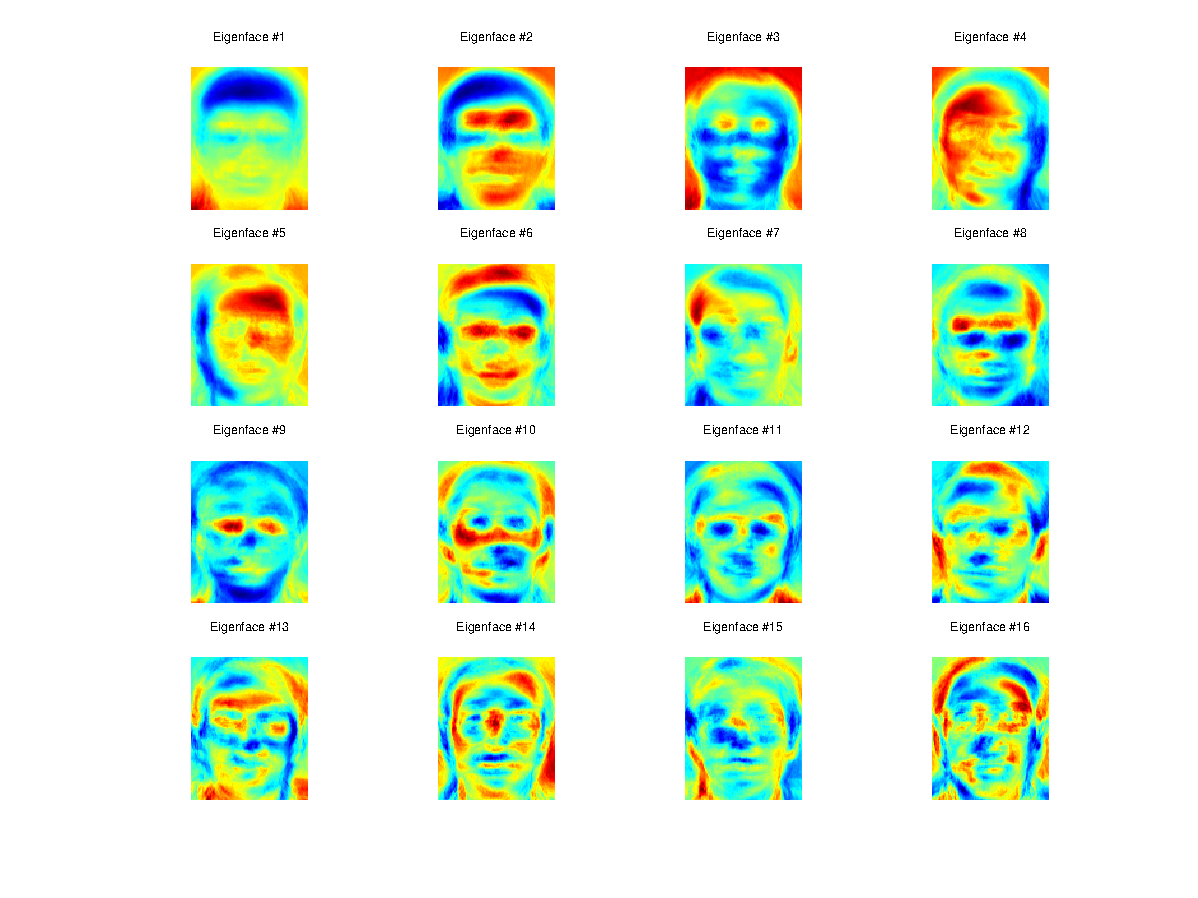
\includegraphics[scale=0.6]{img/eigenfaces/octave_pca_eigenfaces}
\end{center}
\else
	\begin{center}
		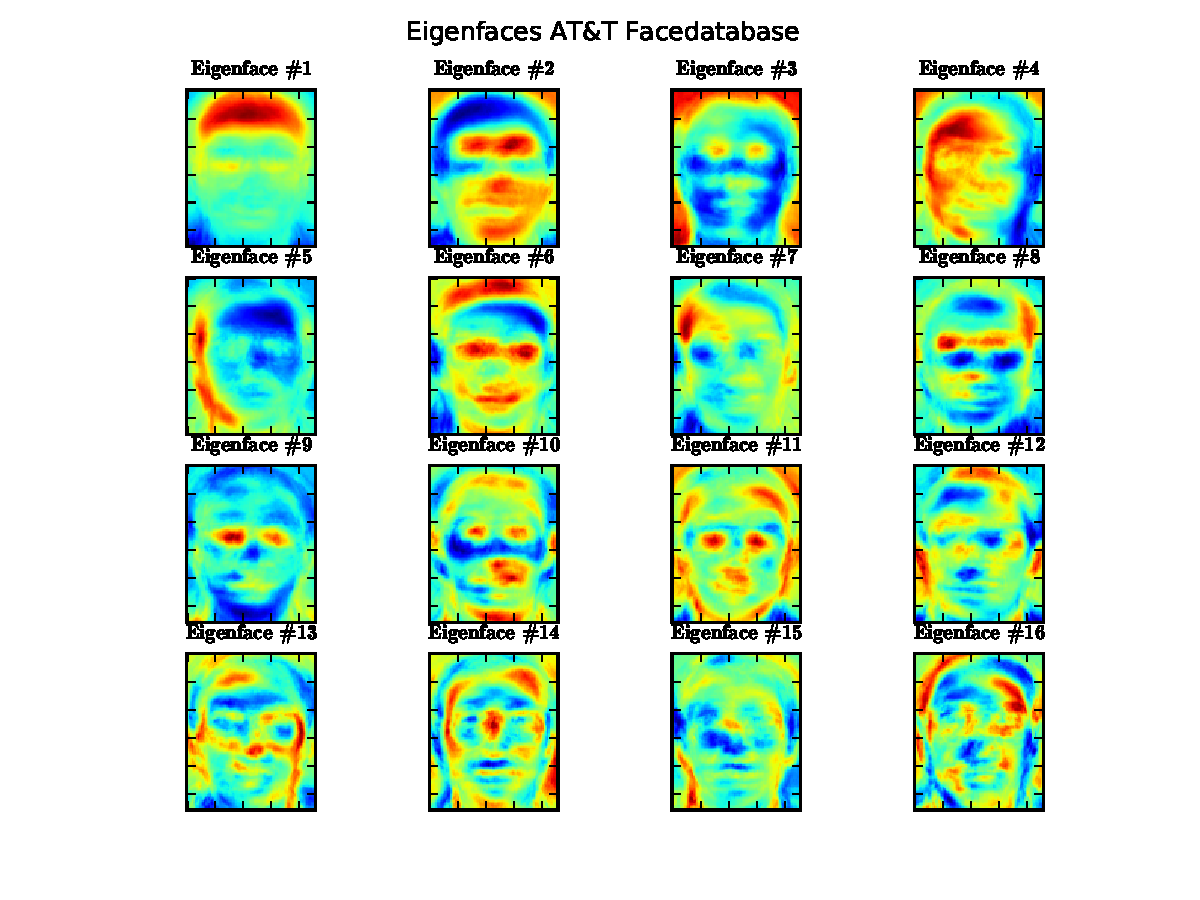
\includegraphics[scale=0.6]{img/eigenfaces/python_pca_eigenfaces}
	\end{center}
\fi

We've already seen in Equation \ref{eqn:pca_reconstruction}, that we can reconstruct a face from its lower dimensional approximation. So let's see how many Eigenfaces are needed for a good reconstruction. I'll do a subplot with $10,30,\ldots,310$ Eigenfaces:

\ifx\python\undefined
	\lstinputlisting[caption={\href{src/m/example\_eigenfaces.m}{src/m/example\_eigenfaces.m} \label{lst:example_pca3}}, language=matlab, linerange={23-36}]{src/m/example_eigenfaces.m}
\else
	\lstinputlisting[caption={\href{src/py/scripts/example\_pca.py}{src/py/scripts/example\_pca.py} \label{lst:example_pca3}}, language=python, linerange={27-40}]{src/py/scripts/example_pca.py}
\fi

10 Eigenvectors are obviously not sufficient for a good image reconstruction, 50 Eigenvectors may already be sufficient to encode important facial features. You'll get a good reconstruction with approximately 300 Eigenvectors for the AT\&T Facedatabase. There are rule of thumbs how many Eigenfaces you should choose for a successful face recognition, but it heavily depends on the input data. \cite{zhao2003frl} is a good point to start researching for this.

\ifx\python\undefined
	\begin{center}
		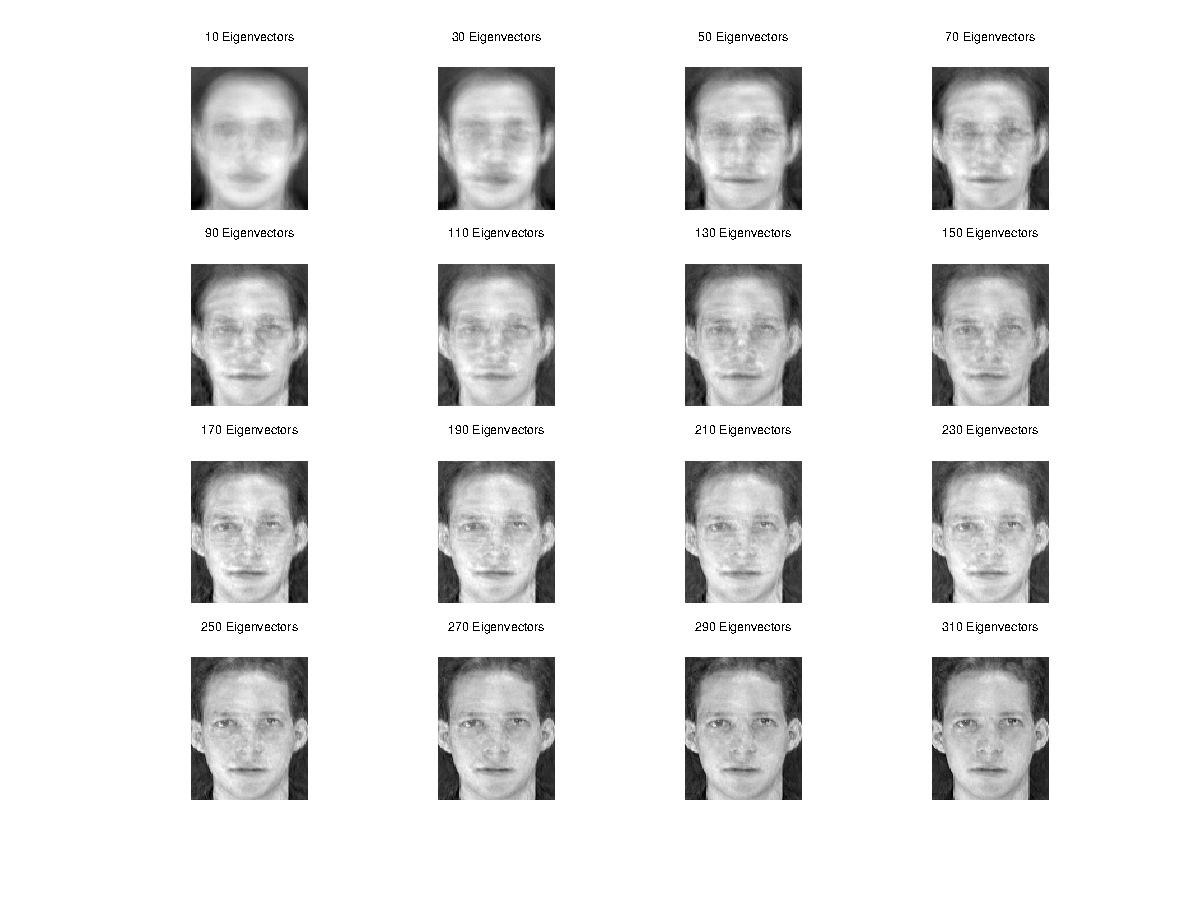
\includegraphics[scale=0.6]{img/eigenfaces/octave_pca_reconstruction}
	\end{center}
\else
	\begin{center}
		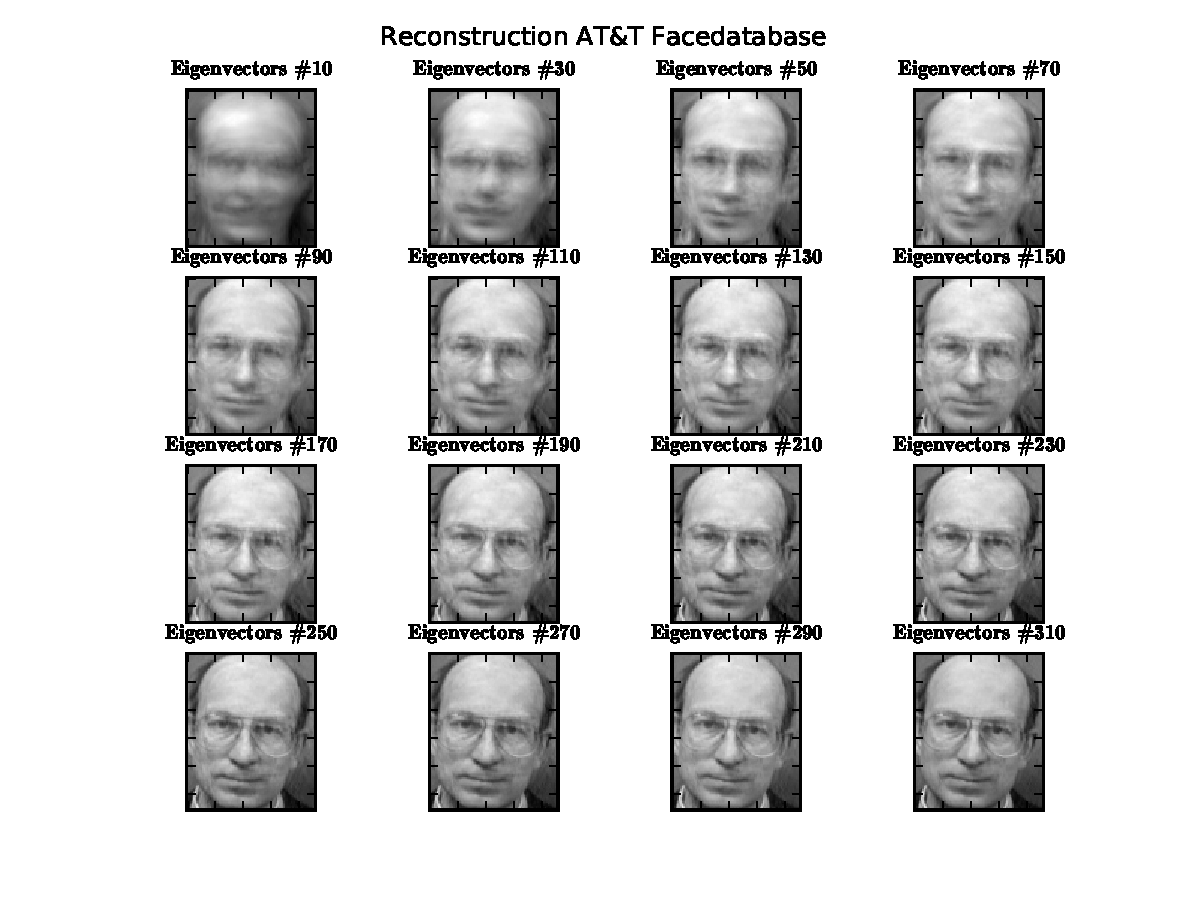
\includegraphics[scale=0.6]{img/eigenfaces/python_pca_reconstruction}
	\end{center}
\fi

\ifx\python\undefined
	The k-Nearest Neighbor matching is left out for this example. Please see the GNU Octave/MATLAB code at \url{https://github.com/bytefish/facerec/tree/master/m} to see how it is implemented, it's all there.
\else
	\subsubsection{The Eigenfaces Method in Python}
	Now we have got everything to implement the Eigenfaces method. \href{http://www.python.org}{Python} is an object oriented programming language, so is our Eigenfaces model. Let's recap... The Eigenfaces method is basically a Pricipal Component Analysis with a Nearest Neighbor model. Some publications report about the influence of the distance metric, so various distance metrics for the Nearest Neighbor search should be supported. It's easy, let's get it done. 
	
	Listing \ref{lst:distance_base} defines \lstinline|AbstractDistance| as the abstract base class for each distance metric. Every subclass must override the call operator \lstinline|__call__|, as shown for the Euclidean Distance and the Negated Cosine Distance. If you search for more distance metrics, please have a look \url{https://www.github.com/bytefish/facerec}.
	
	\lstinputlisting[caption={\href{src/py/tinyfacerec/distance.py}{src/py/tinyfacerec/distance.py} \label{lst:distance_base}}, language=python]{src/py/tinyfacerec/distance.py}
	
	The Eigenfaces and Fisherfaces method both share common methods, so we'll define a base prediction model in Listing \ref{lst:eigenfaces_base_model}. I don't want to do a full k-Nearest Neighbor implementation here, because (1) the number of neighbors doesn't really matter for both methods and (2) it would confuse people. If you are implementing it in a language of your choice, you should really separate the feature extraction from the classification, a real generic approach is given in my \href{https://www.github.com/bytefish/facerec}{facerec} framework. However, feel free to extend these classes for your needs.
	
	\lstinputlisting[caption={\href{src/py/tinyfacerec/model.py}{src/py/tinyfacerec/model.py} \label{lst:eigenfaces_base_model}}, language=python, linerange={1-28}]{src/py/tinyfacerec/model.py}

	Listing \ref{lst:eigenfaces_eigenfaces_model} then subclasses the \lstinline|EigenfacesModel| from the \lstinline|BaseModel|. Only the \lstinline|compute| method needs to be overriden with our specific feature extraction.
	
	\lstinputlisting[caption={\href{src/py/tinyfacerec/model.py}{src/py/tinyfacerec/model.py} \label{lst:eigenfaces_eigenfaces_model}}, language=python, linerange={30-41}]{src/py/tinyfacerec/model.py}
	
		Once the \lstinline|EigenfacesModel| is defined, it can be used to learn the Fisherfaces and generate predictions. In the following Listing \ref{lst:example_model_eigenfaces} we'll load the Yale Facedatabase A and perform a prediction on the first image.
		
	\lstinputlisting[caption={\href{src/py/scripts/example\_model\_eigenfaces.py}{src/py/scripts/example\_model\_eigenfaces.py} \label{lst:example_model_eigenfaces}}, language=python]{src/py/scripts/example_model_eigenfaces.py}

\fi

\subsection{Fisherfaces}

\label{ssection:fisherfaces}

The Linear Discriminant Analysis was invented by the great statistician \href{http://en.wikipedia.org/wiki/Ronald_Fisher}{Sir R. A. Fisher}, who successfully used it for classifying flowers in his 1936 paper \textit{The use of multiple measurements in taxonomic problems} \cite{Fisher36}. But why do we need another dimensionality reduction method, if the Principal Component Analysis (PCA) did such a good job? 

The PCA finds a linear combination of features that maximizes the total variance in data. While this is clearly a powerful way to represuccsent data, it doesn't consider any classes and so a lot of discriminative information may be lost when throwing components away. Imagine a situation where the variance is generated by an external source, let it be the light. The components identified by a PCA do not necessarily contain any discriminative information at all, so the projected samples are smeared together and a classification becomes impossible.

In order to find the combination of features that separates best between classes the Linear Discriminant Analysis maximizes the ratio of between-classes to within-classes scatter. The idea is simple: same classes should cluster tightly together, while different classes are as far away as possible from each other. This was also recognized by \href{http://www.cs.columbia.edu/~belhumeur/}{Belhumeur}, \href{http://www.ece.ucsb.edu/~hespanha/}{Hespanha} and \href{http://cseweb.ucsd.edu/~kriegman/}{Kriegman} and so they applied a Discriminant Analysis to face recognition in \cite{belhumeru97}. 

\begin{figure}
	\begin{center}
		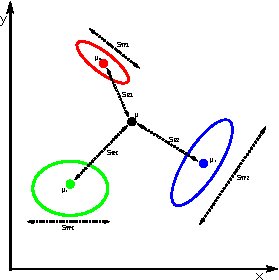
\includegraphics[scale=1.70]{img/fisherfaces/multiclasslda}
		\captionof{figure}{This figure shows the scatter matrices $S_{B}$ and $S_{W}$ for a 3 class problem. $\mu$ represents the total mean and $[\mu_{1},\mu_{2},\mu_{3}]$ are the class means.}
		\label{fig:scatter_matrices}
	\end{center}
\end{figure}

\subsubsection{Algorithmic Description}

Let $X$ be a random vector with samples drawn from $c$ classes:

\begin{eqnarray}
X & = & \{X_1,X_2,\ldots,X_c\} \\
X_i & = & \{x_1, x_2, \ldots, x_n\}
\end{eqnarray}

The scatter matrices $S_{B}$ and $S_{W}$ are calculated as:

% between-classes scatter
\begin{eqnarray}
\label{eqn:scatter_matrices}
S_{B} & = & \sum_{i=1}^{c} N_{i} (\mu_i - \mu)(\mu_i - \mu)^{T} \\
S_{W} & = & \sum_{i=1}^{c} \sum_{x_{j} \in X_{i}} (x_j - \mu_i)(x_j - \mu_i)^{T}
\end{eqnarray}

, where $\mu$ is the total mean:

\begin{equation}
\mu = \frac{1}{N} \sum_{i=1}^{N} x_i
\end{equation}

And $\mu_i$ is the mean of class $i \in \{1,\ldots,c\}$:

% Class-Average
\begin{equation}
\mu_i = \frac{1}{|X_i|} \sum_{x_j \in X_i} x_j
\end{equation}

Fisher's classic algorithm now looks for a projection $W$, that maximizes the class separability criterion:

\begin{equation}
W_{opt} = \operatorname{arg\,max}_{W} \frac{|W^T S_B W|}{|W^T S_W W|}
\end{equation}

Following \cite{belhumeru97}, a solution for this optimization problem is given by solving the General Eigenvalue Problem:

\begin{eqnarray}
\label{eqn:general_eigenwert}
S_{B} v_{i} & = & \lambda_{i} S_w v_{i} \nonumber \\
S_{W}^{-1} S_{B} v_{i} & = & \lambda_{i} v_{i}
\end{eqnarray}

There's one problem left to solve: The rank of $S_{W}$ is at most $(N-c)$, with $N$ samples and $c$ classes. In pattern recognition problems the number of samples $N$ is almost always samller than the dimension of the input data (the number of pixels), so the scatter matrix $S_{W}$ becomes singular (see \cite{Raudys1991}). In \cite{belhumeru97} this was solved by performing a Principal Component Analysis on the data and projecting the samples into the $(N-c)$-dimensional space. A Linear Discriminant Analysis was then performed on the reduced data, because $S_{W}$ isn't singular anymore.

The optimization problem can be rewritten as:

\begin{eqnarray}
W_{pca} & = & \operatorname{arg\,max}_{W} |W^T S_T W| \\
W_{fld} & = & \operatorname{arg\,max}_{W} \frac{|W^T W_{pca}^T S_{B} W_{pca} W|}{|W^T W_{pca}^T S_{W} W_{pca} W|}
\end{eqnarray}

The transformation matrix $W$, that projects a sample into the $(c-1)$-dimensional space is then given by:

\begin{equation} \label{eqn:fisherfaces}
W = W_{fld}^{T} W_{pca}^{T}
\end{equation}

One final note: Although $S_{W}$ and $S_{B}$ are symmetric matrices, the product of two symmetric matrices is not necessarily symmetric. so you have to use an eigenvalue solver for general matrices. OpenCV's \href{http://opencv.willowgarage.com/documentation/cpp/operations_on_arrays.html#cv-eigen}{cv::eigen} only works for symmetric matrices in its current version; since eigenvalues and singular values aren't equivalent for non-symmetric matrices you can't use a Singular Value Decomposition (SVD) either.

\subsubsection{Example}

\label{ssection:example_fisherfaces}

Translating the Linear Discriminant Analysis to \ifx\python\undefined \href{http://www.gnu.org/software/octave/}{GNU Octave}/\href{http://www.mathworks.com}{MATLAB} \else \href{http://www.python.org}{Python}\fi is almost trivial again, see Listing \ref{lst:lda}. For projecting and reconstructing from the basis you can use the functions from Listing \ref{lst:project} and \ref{lst:reconstruct}.
\ifx\python\undefined
	\lstinputlisting[caption={\href{src/m/lda.m}{src/m/lda.m} \label{lst:lda}}, language=matlab]{src/m/lda.m}
\else
		\lstinputlisting[caption={\href{src/py/tinyfacerec/subspace.py}{src/py/tinyfacerec/subspace.py} \label{lst:lda}}, language=python, linerange={39-58}]{src/py/tinyfacerec/subspace.py}
\fi

The functions to perform a PCA (Listing \ref{lst:pca}) and LDA (Listing \ref{lst:lda}) are now defined, so we can go ahead and implement the Fisherfaces from Equation \ref{eqn:fisherfaces}. 

\ifx\python\undefined
	\lstinputlisting[caption={\href{src/m/fisherfaces.m}{src/m/fisherfaces.m} \label{lst:fisherfaces}}, language=matlab]{src/m/fisherfaces.m}
\else
	\lstinputlisting[caption={\href{src/py/tinyfacerec/subspace.py}{src/py/tinyfacerec/subspace.py} \label{lst:fisherfaces}}, language=python, linerange={60-67}]{src/py/tinyfacerec/subspace.py}
\fi

For this example I am going to use the Yale Facedatabase A, just because the plots are nicer. Each Fisherface has the same length as an original image, thus it can be displayed as an image. We'll again load the data, learn the Fisherfaces and make a subplot of the first 16 Fisherfaces.

\ifx\python\undefined
	\lstinputlisting[caption={\href{src/m/example\_fisherfaces.m}{src/m/example\_fisherfaces.m} \label{lst:example_fisherfaces_fisherfaces}}, language=matlab, linerange={1-23}]{src/m/example_fisherfaces.m}
\else
	\lstinputlisting[caption={\href{src/py/scripts/example\_fisherfaces.py}{src/py/scripts/example\_fisherfaces.py} \label{lst:example_fisherfaces_fisherfaces}}, language=python, linerange={1-23}]{src/py/scripts/example_fisherfaces.py}
\fi

The Fisherfaces method learns a class-specific transformation matrix, so the they do not capture illumination as obviously as the Eigenfaces method. The Discriminant Analysis instead finds the facial features to discriminate between the persons. It's important to mention, that the performance of the Fisherfaces heavily depends on the input data as well. Practically said: if you learn the Fisherfaces for well-illuminated pictures only and you try to recognize faces in bad-illuminated scenes, then method is likely to find the wrong components (just because those features may not be predominant on bad illuminated images). This is somewhat logical, since the method had no chance to learn the illumination.

\ifx\python\undefined
	\begin{center}
		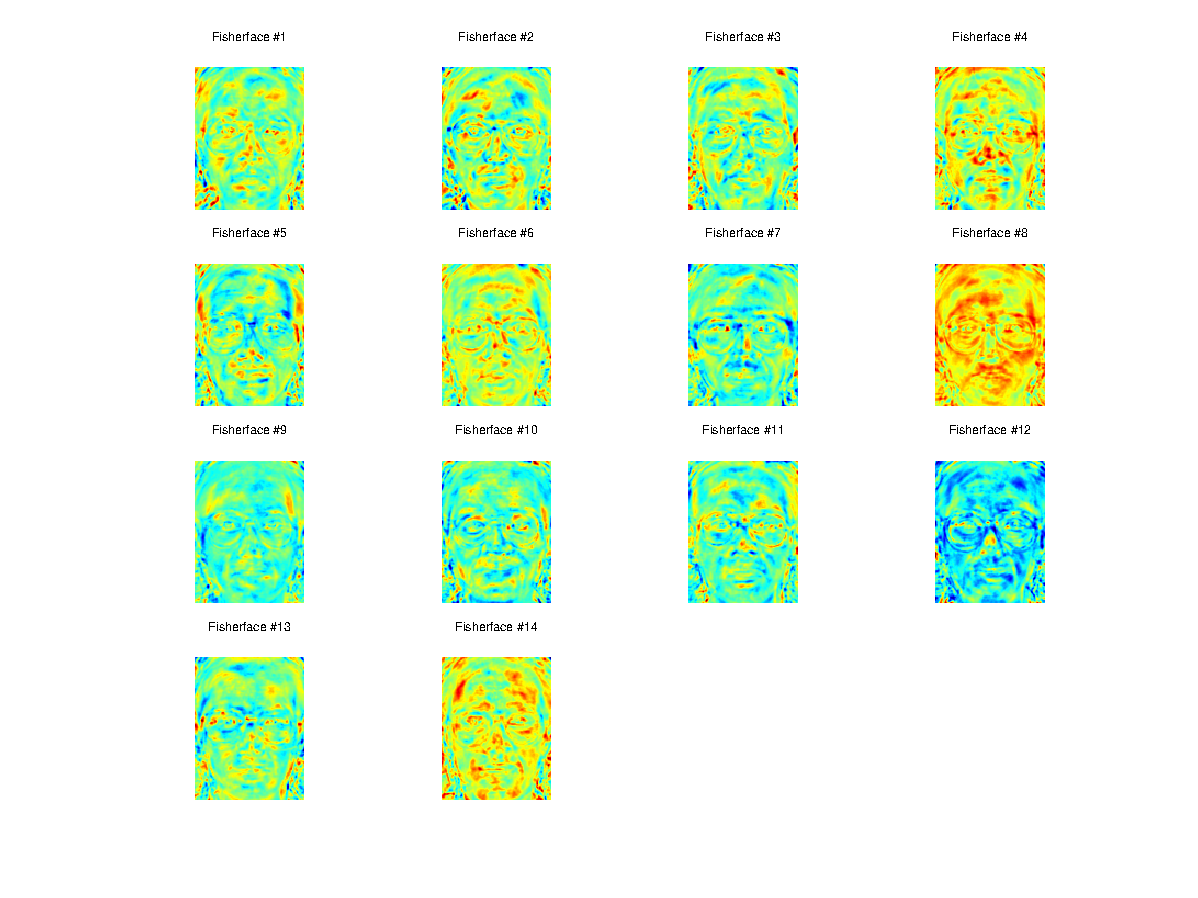
\includegraphics[scale=0.6]{img/fisherfaces/octave_fisherfaces_fisherfaces}
	\end{center}
\else
	\begin{center}
		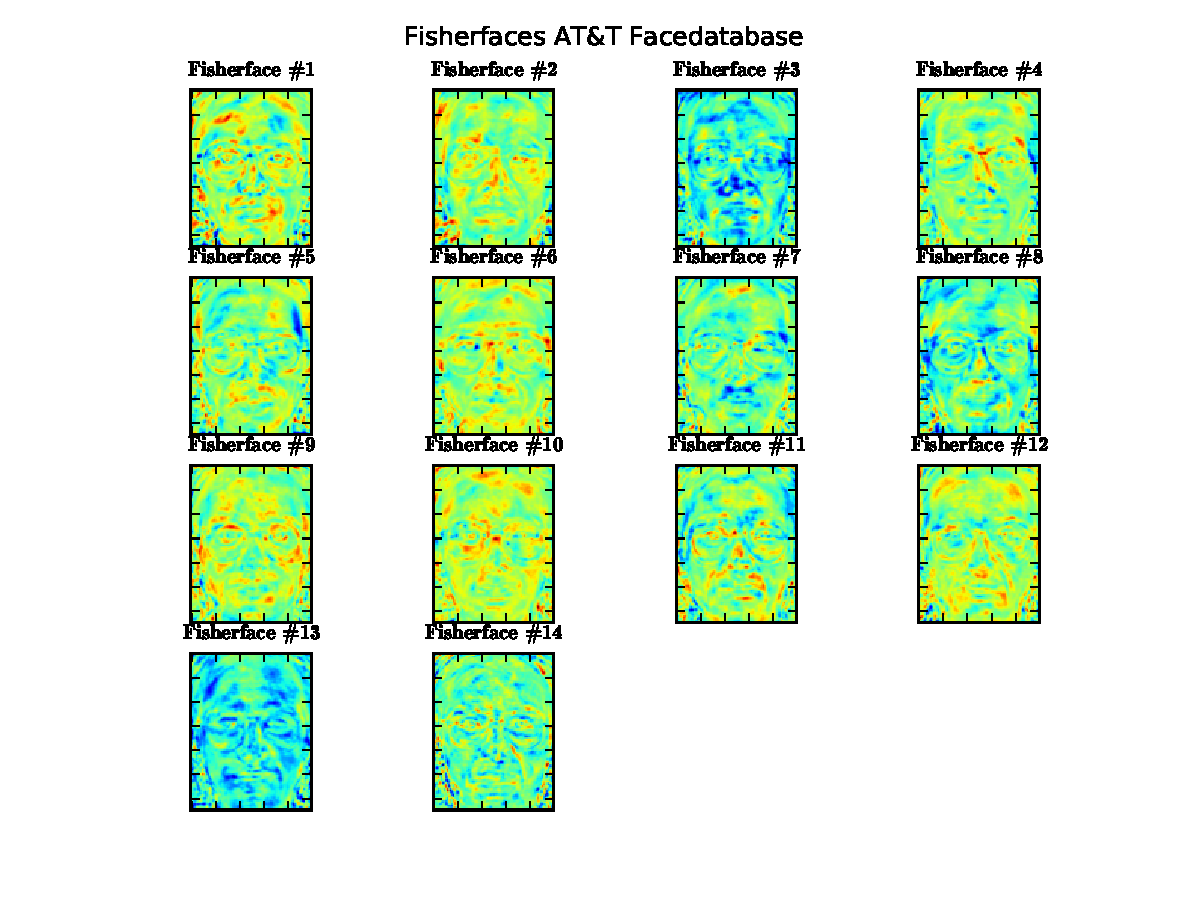
\includegraphics[scale=0.6]{img/fisherfaces/python_fisherfaces_fisherfaces}
	\end{center}
\fi

The Fisherfaces allow a reconstruction of the projected image, just like the Eigenfaces did. But since we only identified the features to distinguish between subjects, you can't expect a nice approximation of the original image. We can rewrite Listing \ref{lst:example_pca3} for the Fisherfaces method into Listing \ref{lst:example_fisherfaces_reconstruction}, but this time we'll project the sample image onto each of the Fisherfaces instead. So you'll have a visualization, which features each Fisherface describes.

\ifx\python\undefined
	\lstinputlisting[caption={\href{src/m/example\_fisherfaces.m}{src/m/example\_fisherfaces.m} \label{lst:example_fisherfaces_reconstruction}}, language=matlab, linerange={28-40}]{src/m/example_fisherfaces.m}
\else
	\lstinputlisting[caption={\href{src/py/scripts/example\_fisherfaces.py}{src/py/scripts/example\_fisherfaces.py} \label{lst:example_fisherfaces_reconstruction}}, language=python, linerange={25-36}]{src/py/scripts/example_fisherfaces.py}
\fi


\ifx\python\undefined
	\begin{center}
		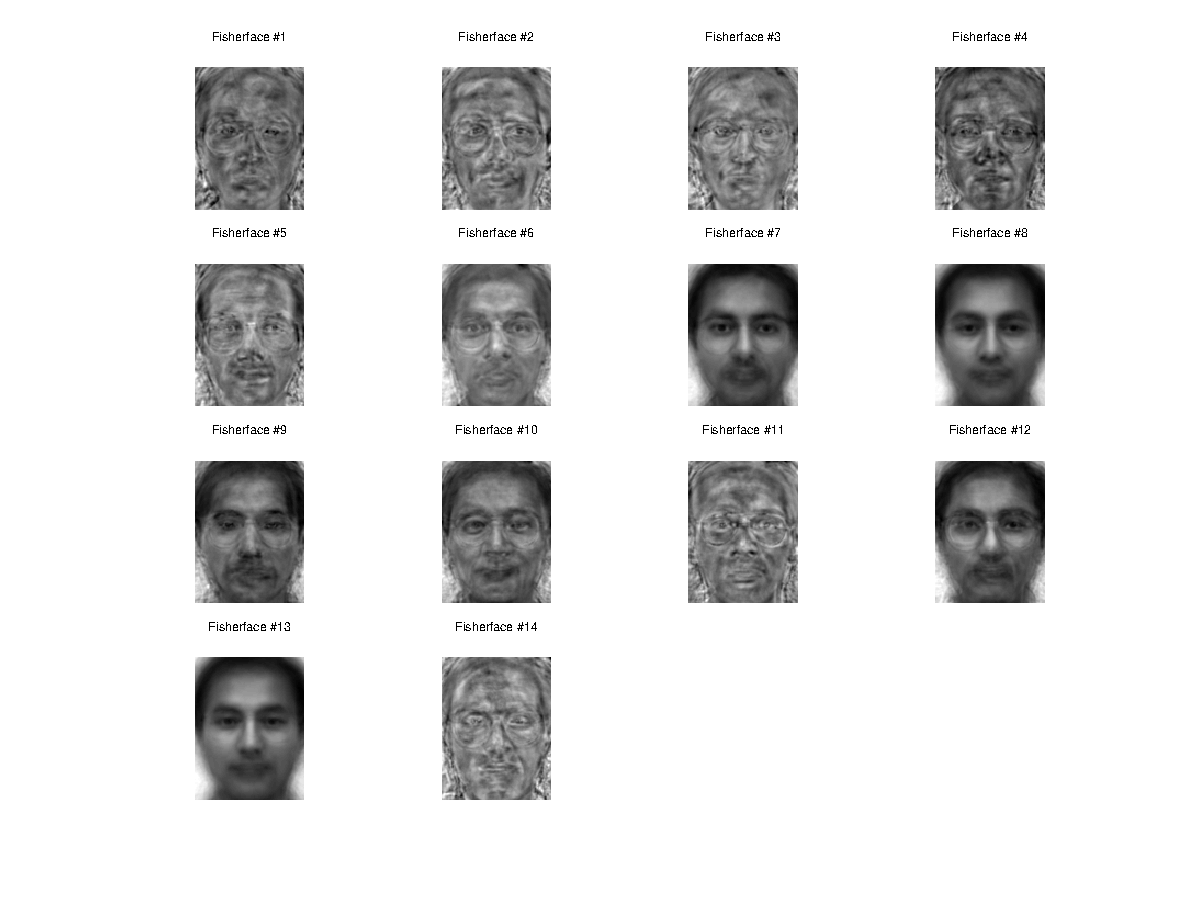
\includegraphics[scale=0.6]{img/fisherfaces/octave_fisherfaces_reconstruction}
	\end{center}
\else
	\begin{center}
		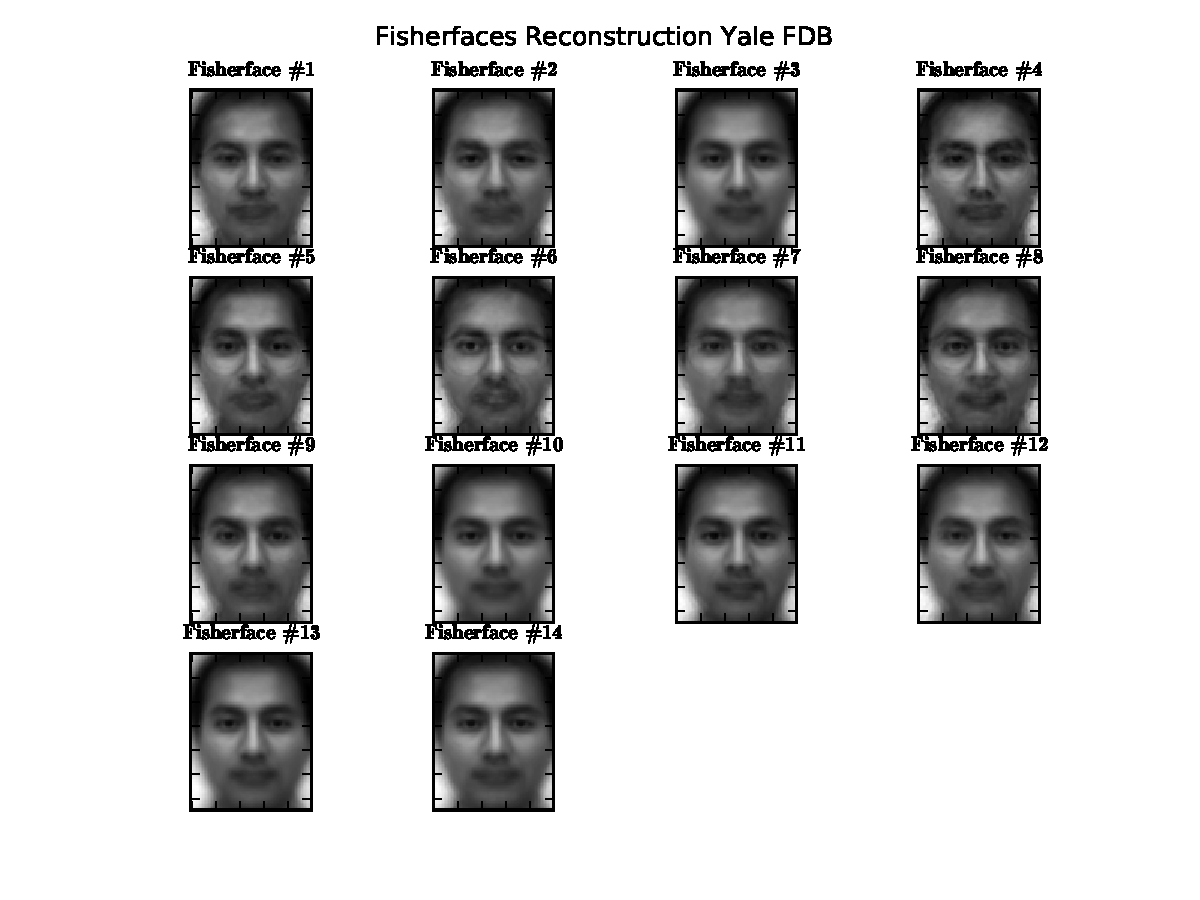
\includegraphics[scale=0.6]{img/fisherfaces/python_fisherfaces_reconstruction}
	\end{center}
\fi

\ifx\python\undefined
	The k-Nearest Neighbor matching is left out for this example. Please see the GNU Octave/MATLAB code at \url{https://github.com/bytefish/facerec/tree/master/m} to see how it is implemented, it's all there.
\else
	\subsubsection{The Fisherfaces Method in Python}
	The implementation details are not repeated in this section. For the Fisherfaces method a similar model to the \lstinline|EigenfacesModel| in Listing \ref{lst:eigenfaces_eigenfaces_model} must be defined.
		
	\lstinputlisting[caption={\href{src/py/tinyfacerec/model.py}{src/py/tinyfacerec/model.py} \label{lst:eigenfaces_eigenfaces_model}}, language=python, linerange={43-54}]{src/py/tinyfacerec/model.py}
	
		Once the \lstinline|FisherfacesModel| is defined, it can be used to learn the Fisherfaces and generate predictions. In the following Listing \ref{lst:example_model_fisherfaces} we'll load the Yale Facedatabase A and perform a prediction on the first image.
		
	\lstinputlisting[caption={\href{src/py/scripts/example\_model\_fisherfaces.py}{src/py/scripts/example\_model\_fisherfaces.py} \label{lst:example_model_fisherfaces}}, language=python]{src/py/scripts/example_model_fisherfaces.py}

\fi



\section{Face Recognition with OpenCV2 C++ API}

The C++ API of OpenCV2 closely resembles the \ifx\python\undefined \href{http://www.gnu.org/software/octave/}{GNU Octave}/\href{http://www.mathworks.com}{MATLAB} \else \href{http://www.python.org}{Python} \fi code we've written in section \ref{ssection:example_eigenfaces} and \ref{ssection:example_fisherfaces}. If you have prototyped it, you won't have a great problem translating it to OpenCV2. I personally think you don't need a book to learn about the OpenCV2 C++ API. There's a lot of documentation coming with OpenCV, just have a look into the \lstinline|doc| folder of your OpenCV installation. The easiest way to get started is the \textit{OpenCV Cheat Sheet (C++)} (\lstinline|opencv_cheatsheet.pdf|), because it shows you how to use all the functions with examples. The \textit{The OpenCV Reference Manual} (\lstinline|opencv2refman.pdf|) is the definite guide to the API (500+ pages). Of course, you'll need a book or other literature for understanding computer vision algorithms - I can't give an introduction to this here.

\subsection{Downloading and Building the Source Code}

Only a high-level description of the implementation is given, because pasting the complete code doesn't make any sense. The source code is available at \url{http://www.github.com/bytefish/opencv} and none of the projects have additional dependencies.

\begin{itemize}
	\item \textbf{Eigenfaces}: \url{https://github.com/bytefish/opencv/tree/master/eigenfaces}
	\item \textbf{Fisherfaces}: \url{https://github.com/bytefish/opencv/tree/master/lda}
\end{itemize}

If you want to clone both projects with \href{http://git-scm.com/}{git} then issue:

\begin{lstlisting}
git clone git@github.com:bytefish/opencv.git
\end{lstlisting}

However, if you don't have \href{http://git-scm.com/}{git} on your system you can download both projects as zip or tarball:

\begin{itemize}
	\item \textbf{zip} \url{https://github.com/bytefish/opencv/zipball/master}
	\item \textbf{tar} \url{https://github.com/bytefish/opencv/tarball/master}
\end{itemize}

Building the demo executables is then as simple as (assuming you are in a projects folder):

\begin{lstlisting}
mkdir build
cd build
cmake ..
make
./eigenfaces /path/to/csv.ext
\end{lstlisting}

Or if you are on Windows with MinGW you would do:

\begin{lstlisting}
mkdir build
cd build
cmake -G "MinGW Makefiles" ..
mingw32-make
eigenfaces.exe /path/to/csv.ext
\end{lstlisting}

Please make sure to read the \textit{README.markdown} coming with each project!

\subsection{Reading in the face images}

\lstset{language=,}

OpenCV can read data from various video sources and image types, you can start your research with the documentation on \href{http://opencv.willowgarage.com/documentation/cpp/reading_and_writing_images_and_video.html}{Reading and Writing Images and Video}. I needed to read images from different folders for a project and I don't know a simpler approach than reading from a CSV file (if you know a simpler approach, please ping me):

\begin{lstlisting}[language=c++]
void read_csv(const string& filename, vector<Mat>& images, vector<int>& labels) {
  std::ifstream file(filename.c_str(), ifstream::in);
  if(!file)
    throw std::exception();
  std::string line, path, classlabel;
  // for each line
  while (std::getline(file, line)) {
    // get current line
    std::stringstream liness(line);
    // split line
    std::getline(liness, path, ';');
    std::getline(liness, classlabel);
    // push pack the data
    images.push_back(imread(path,0));
    labels.push_back(atoi(classlabel.c_str()));
  }
}
\end{lstlisting}

Some people had questions about the usage of the executables, mainly concerned with reading the images and the corresponding labels from a CSV file. Basically all the CSV file needs to contain are lines composed of a \textit{filename} followed by a \textit{;} followed by the \textit{label} (as integer number), making up a line like this: \lstinline|/path/to/image;0|. So if the AT\&T Facedatabase is extracted to \lstinline|/home/philipp/facerec/data/at| the CSV file has to look like this:

\begin{lstlisting}
/home/philipp/facerec/data/at/s1/1.pgm;0
/home/philipp/facerec/data/at/s1/2.pgm;0
[...]
/home/philipp/facerec/data/at/s2/1.pgm;1
/home/philipp/facerec/data/at/s2/2.pgm;1
[...]
/home/philipp/facerec/data/at/s40/1.pgm;39
/home/philipp/facerec/data/at/s40/2.pgm;39
\end{lstlisting}

Think of the label as the subject (the person) you want to recognize. You don't need to take care about the order of the labels, just make sure the same subjects (persons) belong to the same (unique) label.\footnote{The CSV file for the AT\&T Database comes with this document.} I'll now show the definition of the classes and a source code listing, that shows how to use the classes. I think the code answers most of the questions already.

\subsection{Eigenfaces}

\subsubsection{Definiton}
\begin{lstlisting}[language=c++]
class Eigenfaces {
public:
  //! Initialize an empty Eigenfaces model with num_components = 0 
  //   and dataAsRow = true.
  Eigenfaces();
  //! Initialize a Eigenfaces model for num_components and dataAsRow.
  Eigenfaces(int num_components, bool dataAsRow = true);
  //! compute the eigenfaces for data (given in src) and labels, keep 
  //   num_components principal components. Pass dataAsRow = true, if 
  //   the observations are given by row, false if given by column.
  Eigenfaces(const vector<Mat>& src, 
      const vector<int>& labels, 
      int num_components = 0, 
      bool dataAsRow = true);
  //! compute the eigenfaces for data (given in src) and labels, keep 
  //   num_components principal components. Pass dataAsRow = true, if 
  //   the observations are given by row, false if given by column.
  Eigenfaces(const Mat& src, 
      const vector<int>& labels, 
      int num_components = 0, 
      bool dataAsRow = true);
  //! compute the eigenfaces for data (given in src) and labels      
  void compute(const vector<Mat>& src, const vector<int>& labels);
  //! compute the eigenfaces for data (given in src) and labels
  void compute(const Mat& src, const vector<int>& labels);
  //! get a prediction for a given a sample
  int predict(const Mat& src);
  //! project a sample
  Mat project(const Mat& src);
  //! reconstruct a sample
  Mat reconstruct(const Mat& src);
  //! getter
  Mat eigenvectors() const;
  Mat eigenvalues() const;
  Mat mean() const;
};
\end{lstlisting}

\subsubsection{Example}
\begin{lstlisting}[language=c++]
// ...
// include the eigenfaces
#include "eigenfaces.hpp"
// ...
int main(int argc, char *argv[]) {
  // the samples and corresponding labels (classes/subjects/...)
  vector<Mat> images;
  vector<int> labels;
  // read in images and labels
  string fn_csv = string("/path/to/your/csv.ext");
  // read in the images
  try {
    read_csv(fn_csv, images, labels);
  } catch(exception& e) {
    cerr << "Error opening file \"" << fn_csv << "\"." << endl;
    exit(1);
  }
  // get width and height of the samples
  int width = images[0].cols;
  int height = images[0].rows;
  // get a test sample
  Mat testSample = images[images.size()-1];
  int testLabel = labels[labels.size()-1];
  // ... and delete it from training samples
  images.pop_back();
  labels.pop_back();
  // num_components eigenfaces 
  int num_components = 80;
  // compute the eigenfaces
  Eigenfaces eigenfaces(images, labels, num_components);
  // get a prediction (recognize a face)
  int predicted = eigenfaces.predict(testSample);
  cout << "actual=" << testLabel << " / predicted=" << predicted << endl;
  // see the reconstruction with num_components
  Mat p = eigenfaces.project(images[0].reshape(1,1));
  Mat r = eigenfaces.reconstruct(p);
  // see the reconstruction with num_components eigenfaces
  imshow("original", images[0]);
  imshow("reconstruction", toGrayscale(r.reshape(1, height)));
  // get the eigenvectors
  Mat W = eigenfaces.eigenvectors();
  // show first 10 eigenfaces
  for(int i = 0; i < 10; i++) {
    Mat ev = W.col(i).clone();
    imshow(num2str(i), toGrayscale(ev.reshape(1, height)));
  }
  // ...
}
\end{lstlisting}

\subsection{Fisherfaces}

\subsubsection{Definition}
\begin{lstlisting}[language=c++]
class Fisherfaces {

public:
  //! Initialize an empty Eigenfaces model with num_components = 0
  //   and dataAsRow = true.
  Fisherfaces();
  //! Initialize a Fisherfaces model for num_components and dataAsRow.
  Fisherfaces(int num_components, 
      bool dataAsRow = true);
  //! compute the fisherfaces for data (given in src) and labels, keep 
  //   num_components discriminants. Pass dataAsRow = true, if the 
  //   observations are given by row, false if given by column.
  Fisherfaces(const vector<Mat>& src, 
      const vector<int>& labels,
      int num_components = 0,
      bool dataAsRow = true);
  //! compute the fisherfaces for data (given in src) and labels, keep 
  //   num_components discriminants. Pass dataAsRow = true, if the 
  //   observations are given by row, false if given by column.
  Fisherfaces(const Mat& src,
      const vector<int>& labels,
      int num_components = 0,
      bool dataAsRow = true);
  //! compute the fisherfaces for data (given in src) and labels 
  void compute(const Mat& src, const vector<int>& labels);
  //! compute the fisherfaces for data (given in src) and labels 
  void compute(const vector<Mat>& src, const vector<int>& labels);
  //! get a prediction for a given a sample
  int predict(const Mat& src);
  //! project a sample
  Mat project(const Mat& src);
  //! reconstruct a sample
  Mat reconstruct(const Mat& src);
  // getter
  Mat eigenvectors() const;
  Mat eigenvalues() const;
  Mat mean() const;
};
\end{lstlisting}

\subsubsection{Example}
\begin{lstlisting}[language=c++]
// ...
// include the fisherfaces header
#include "fisherfaces.hpp"
// ...
int main(int argc, char *argv[]) {
  // the samples and corresponding labels (classes/subjects/...)
  vector<Mat> images;
  vector<int> labels;
  // read in images and labels
  string fn_csv = string("/path/to/your/csv.ext");
  // read in the images
  try {
    read_csv(fn_csv, images, labels);
  } catch(exception& e) {
    cerr << "Error opening file \"" << fn_csv << "\"." << endl;
    exit(1);
  }
  // get width and height
  int width = images[0].cols;
  int height = images[0].rows;
  // get test instances
  Mat testSample = images[images.size()-1];
  int testLabel = labels[labels.size()-1];
  // ... and delete last element
  images.pop_back();
  labels.pop_back();
  // build the Fisherfaces model
  subspace::Fisherfaces model(images, labels);
  // test model
  int predicted = model.predict(testSample);
  cout << "predicted class = " << predicted << endl;
  cout << "actual class = " << testLabel << endl;
  // get the eigenvectors
  Mat W = model.eigenvectors();
  // show first 10 fisherfaces
  for(int i = 0; i < 10; i++) {
    Mat ev = W.col(i).clone();
    imshow(num2str(i), toGrayscale(ev.reshape(1, height)));
  }
}
\end{lstlisting}

\subsection{Linear Discriminant Analysis}

The Fisherfaces method includes a Linear Discriminant Analysis, so you get this class for free.

\subsubsection{Definition}
\begin{lstlisting}[language=c++]
class LinearDiscriminantAnalysis {

public:
  //! Initialize an empty LDA model with num_components = 0
  //   and dataAsRow = true.
  LinearDiscriminantAnalysis();
  //! Initialize a LDA model for num_components and dataAsRow.
  LinearDiscriminantAnalysis(int num_components, bool dataAsRow = true);
  //! compute the LDA for data (given in src) and labels, keep 
  //   num_components discriminants. Pass dataAsRow = true, if the 
  //   observations are given by row, false if given by column.
  LinearDiscriminantAnalysis(const Mat& src,
      const vector<int>& labels,
      int num_components = 0,
      bool dataAsRow = true);
  //! compute the LDA for data (given in src) and labels, keep 
  //   num_components discriminants. Pass dataAsRow = true, if the 
  //   observations are given by row, false if given by column.
  LinearDiscriminantAnalysis(const vector<Mat>& src,
      const vector<int>& labels,
      int num_components = 0,
      bool dataAsRow = true);
  //! compute the LDA for data (given in src) and labels 
  void compute(const Mat& src, const vector<int>& labels);
  //! compute the LDA for data (given in src) and labels 
  void compute(const vector<Mat>& src, const vector<int>& labels);
  //! project a sample
  Mat project(const Mat& src);
  //! reconstruct a sample
  Mat reconstruct(const Mat& src);
  //! getter
  Mat eigenvectors() const;
  Mat eigenvalues() const;
};
\end{lstlisting}

\subsubsection{Example}
This example is the OpenCV C++ implementation of the tutorial at \url{http://bytefish.de/wiki/pca_lda_with_gnu_octave}. The values found by GNU Octave are reported in the comments. If you want to work through the example yourself, the GNU Octave/MATLAB code is \href{http://bytefish.de/wiki/pca_lda_with_gnu_octave}{given on the wiki page}.

\begin{lstlisting}[language=c++]
// ...
// include the fisherfaces header
#include "fisherfaces.hpp"
// ... or 
//#include "subspace.hpp"

int main(int argc, char *argv[]) {
  // example taken from: http://www.bytefish.de/wiki/pca_lda_with_gnu_octave
  double d[11][2] = {
      {2, 3},
      {3, 4},
      {4, 5},
      {5, 6},
      {5, 7},
      {2, 1},
      {3, 2},
      {4, 2},
      {4, 3},
      {6, 4},
      {7, 6}};
  int c[11] = {0,0,0,0,0,1,1,1,1,1,1};
  // convert into OpenCV representation
  Mat _data = Mat(11, 2, CV_64FC1, d).clone();
  vector<int> _classes(c, c + sizeof(c) / sizeof(int));
  // perform the lda
  subspace::LinearDiscriminantAnalysis lda(_data, _classes);
  // GNU Octave finds the following Eigenvalue:
  //octave> d
  //d =
  //   1.5195e+00
  //
  // Eigen finds the following Eigenvalue:
  // [1.519536390756363]
  //
  // Since there's only 1 discriminant, this is correct.
  cout << "Eigenvalues:" << endl << lda.eigenvalues() << endl;
  // GNU Octave finds the following Eigenvectors:
  //  octave:13> V(:,1)
  //  V =
  //
  //     0.71169  -0.96623
  //    -0.70249  -0.25766
  //
  // Eigen finds the following Eigenvector:
  // [0.7116932742510111;
  //  -0.702490343980524 ]
  //
  cout << "Eigenvectors:" << endl << lda.eigenvectors() << endl;
  // project a data sample onto the subspace identified by LDA
  Mat x = _data.row(0);
  cout << "Projection of " << x << ": " << endl;
  cout << lda.project(x) << endl;
}
\end{lstlisting}

\section{Conclusion}



\appendix
%\input{section/appendix.tex}

\bibliography{bib/facerec}
\bibliographystyle{acm}

\end{document}


